\appendix

\section{Motivating Example: Snapshot Isolation}
\label{appendix:snapshotIsolationExample}



The next program captures serializability through the lens of the \textit{snapshot isolation} consistency model, which is used in various real-world database systems, including \texttt{PostgreSQL}~\cite{postgresql-transaction-iso} and \texttt{CockroachDB}~\cite{cockroachdb-si-docs}, and has been linked to real‐world anomalies (e.g., duplicate‐key errors in the latter~\cite{cockroach-issue-14099}).
%
The depicted program has two nodes (represented by the global variables $N_1$ and $N_2$) which monitor ongoing traffic in the network, and are originally both active, as indicated by their initial values [$N_1=1,N_2=1$].
%
The {\color{ForestGreen}$\blacklozenge_\text{main}$} request takes a snapshot of the system, i.e., locally records the current activation status of each of the two nodes.
%
Then, in the first request, and in any future ones in which both nodes are active, each in-flight request non-deterministically decides which of the two nodes to deactivate, i.e. set [$N_i:=0$], for maintaining overall energy efficiency.
%
The {\color{ForestGreen}$\blacklozenge_\text{main}$} request eventually returns the current sum of active nodes in the system.
%
In order for the system to emulate multiple iterations, our setting also includes two additional requests, {\color{ForestGreen}$\blacklozenge_\text{activate\_n1}$},{\color{ForestGreen}$\blacklozenge_\text{activate\_n2}$} which activate nodes $N_1$ and $N_2$, respectively.
%
We note that the program is not serializable due to the yield operation that appears immediately after the recorded snapshot of the node activation status. One such example for a non-serializable behavior occurs when two {\color{ForestGreen}$\blacklozenge_\text{main}$} requests each record two active monitor nodes and yield; Then, having each request turn off the complement node. As a result of each request operating based on its isolated snapshot of the global state, both monitor nodes can be turned off and we can attain a request with {\color{ForestGreen}$\blacklozenge_\text{main}$}/{\color{red}$\blacklozenge_0$} (for [$N_1+N_2=0+0=0$]).
%
We note that in any serializable execution, no two {\color{ForestGreen}$\blacklozenge_\text{main}$} requests can record both monitors as active, and hence, a response of {\color{red}$\blacklozenge_0$} is unattainable via serializable executions.




\begin{minipage}[t]{1.0\textwidth}
	\begin{lstlisting}[caption={Snapshot-based monitor deactivation (not serializable)},numbers=none]
				// initialize both monitors to be active
				N_1_ACTIVE := 1
				N_2_ACTIVE := 1
				
				request main:
					// take snapshot
					n_1_active_snapshot := N_1_ACTIVE
					n_2_active_snapshot := N_2_ACTIVE
					yield
					
					if (n_1_active_snapshot == 1) and (n_2_active_snapshot == 1):
					// if both nodes active --- choose which one to deactivate 
						if (?): 
							  N_1_ACTIVE := 0
						else:
							  N_2_ACTIVE := 0
						
					return N_1_ACTIVE + N_2_ACTIVE  // total active nodes
					
				
				request activate_n1:
					    N_1_ACTIVE := 1
				
				request activate_n2:
					    N_2_ACTIVE := 1
				
				
			\end{lstlisting}
\end{minipage}

%only 0 in non-serializable runs!

%\todo{start}

%/snapshot_isolation_directly_as_NS_with_yields

%\begin{figure}[h]
%	\centering
%	\includegraphics[width=1.0\linewidth]{plots/snapshot\_isolation\_JSON\_with\_yields.pdf}
%	\caption{Snapshot Isolation with Yields.}
%	\label{fig:snapshotIsolationJsonWithYields}
%\end{figure}
%
%
%
%%/snapshot_isolation_directly_as_NS_without_yields
%
%\begin{figure}[h]
%	\centering
%	\includegraphics[width=1.0\linewidth]{plots/snapshot\_isolation\_JSON\_without\_yields.pdf}
%	\caption{Snapshot Isolation without Yields.}
%	\label{fig:snapshotIsolationJsonWithoutYields}
%\end{figure}


%\todo{maybe we have: (1) a copy of the global automaton; (2) a copy of the local automaton (with yields) with coloring of edges that don't exist in the one without yields}


%\begin{figure}[h]
%	\centering
%	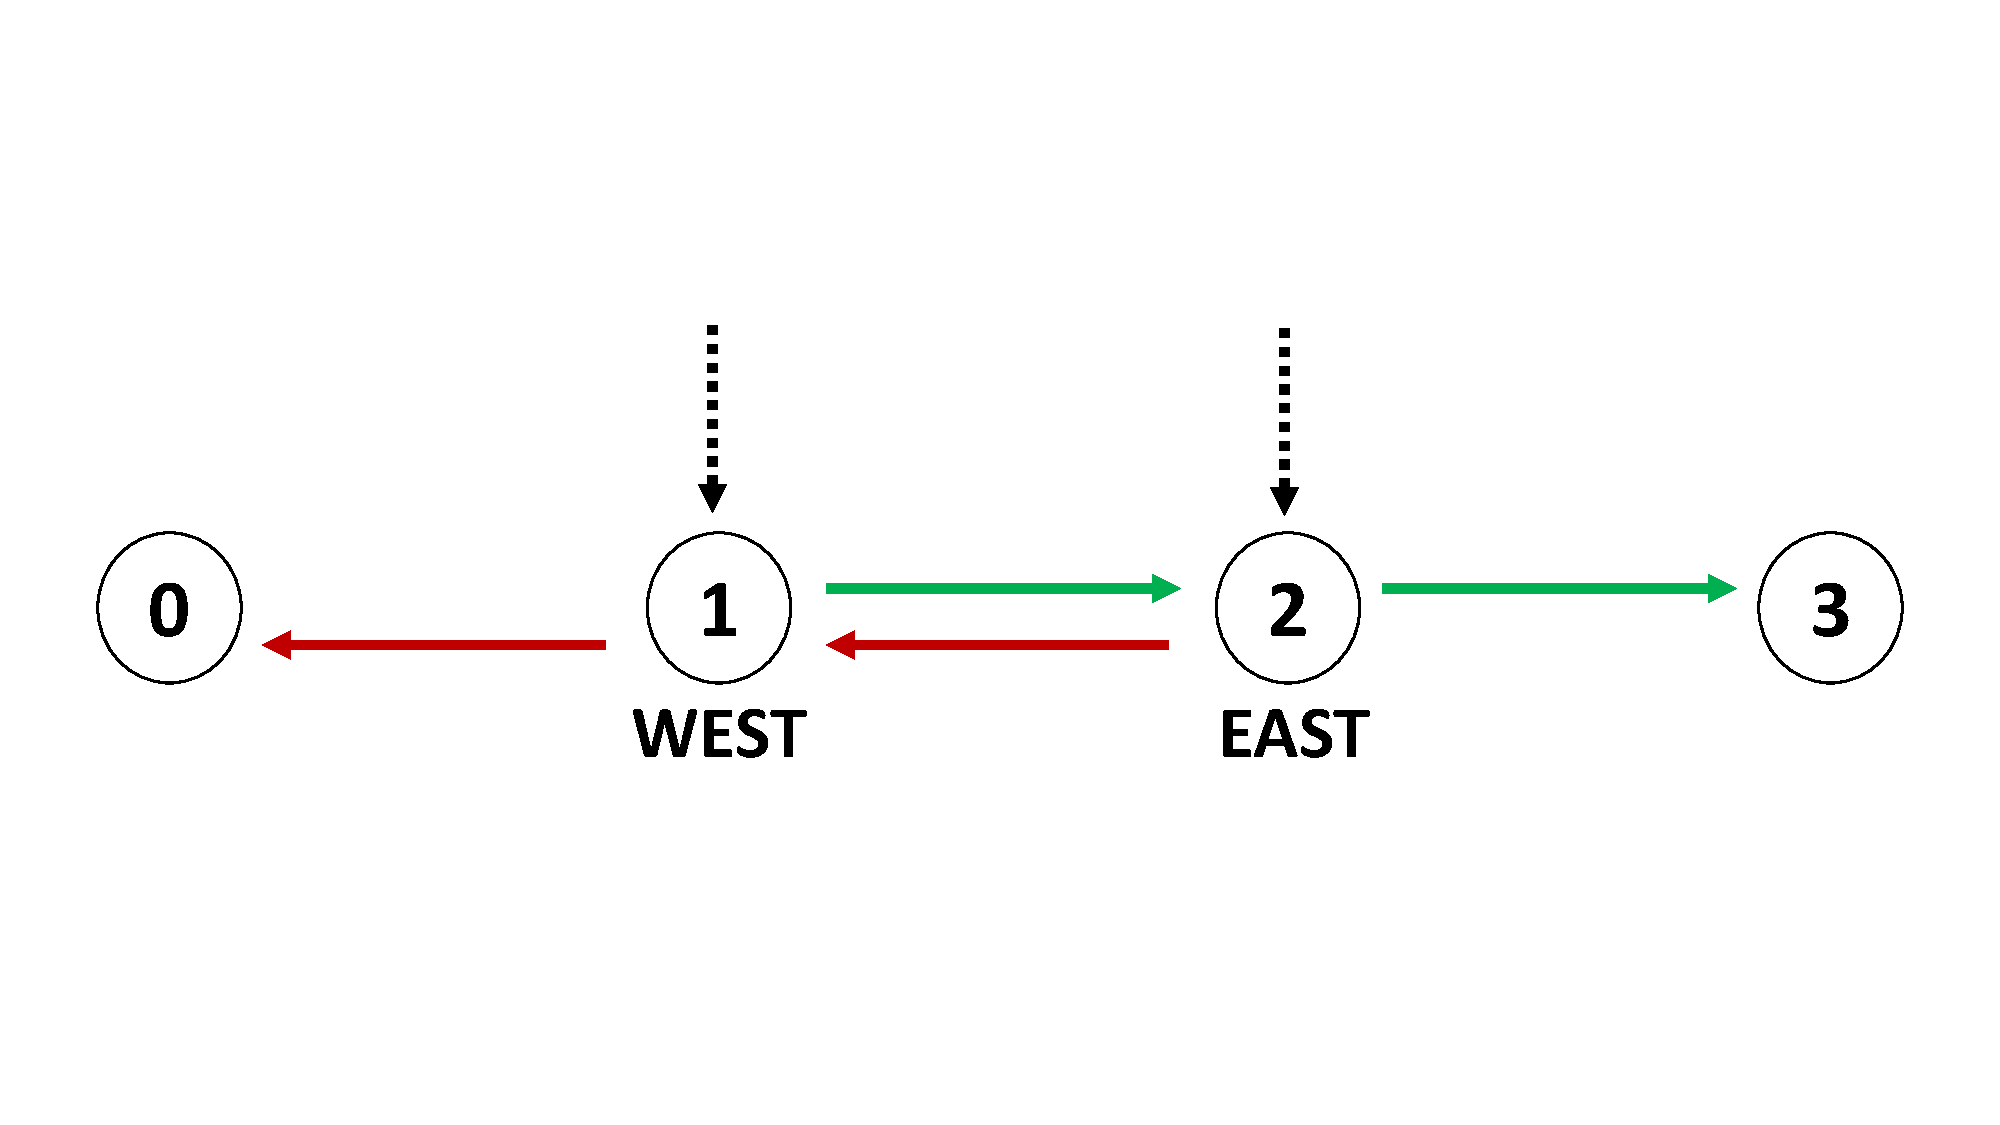
\includegraphics[width=0.65\linewidth]{plots/BgpColoredRouting.pdf}
%	\caption{Routing policy in example 7.}
%	\label{fig:pdfimage}
%\end{figure}

%\newpage
%
%
%example – 8
%
%\noindent
%\begin{minipage}[t]{0.45\textwidth}
%	\begin{lstlisting}[caption={foo (serializable)}]
	%	request foo: 
	%	    if (?):
	%	        X := (X + 2) % 3 
	%	        // no yield
	%	        return X
	%	
	%	    else:
	%	        X := (X + 1) % 3
	%	        // no yield
	%	        return X
	%		\end{lstlisting}
%\end{minipage}
%\hfill
%\begin{minipage}[t]{0.45\textwidth}
%\begin{lstlisting}[caption={foo (non serializable)}]
%request foo: 
%     if (?):
%         X := (X + 2) % 3 
%         yield
%         return X
%
%     else:
%         X := (X + 1) % 3
%         yield
%         return X
%	\end{lstlisting}
%\end{minipage}
%
%One output that is attainable only via non-serializable executions is 
%\[
%\{(foo,1),(foo,1),(foo,1),(foo,3)\}
%\]
%
%
%%\newpage
%
%
%example – 9
%
%\noindent
%\begin{minipage}[t]{0.45\textwidth}
%	\begin{lstlisting}[caption={foo (serializable)}]
%request foo:
%    if(STOP == 0):
%        X := (X + 1) % 4
%
%    yield
%
%    if(STOP == 0):
%        X := (X + 1) % 4
%
%        STOP := ?
%        
%        if(STOP == 1):
%	        return X
%        return 0
%	\end{lstlisting}
%\end{minipage}
%\hfill
%\begin{minipage}[t]{0.45\textwidth}
%	\begin{lstlisting}[caption={foo (non serializable)}]
%request foo:
%    if(STOP == 0):
%        X := (X + 1) % 4
%
%    yield
%
%    if(STOP == 0):
%        X := (X + 2) % 4
%
%        STOP := ?
%        
%        if(STOP == 1):
%	        return X
%        return 0
%	\end{lstlisting}
%\end{minipage}





%\newpage